\documentclass[a4paper, 14pt]{extarticle}
\usepackage{enumitem}
\usepackage{fefutitle}
\usepackage{listings}
\usepackage{xcolor}
\usepackage{amsmath}
\usepackage{graphicx}
\usepackage[justification=centering]{caption}
\usepackage{float}

\lstdefinestyle{mystyle}{
	basicstyle={\small\ttfamily},
	keywordstyle=\color{orange},
	stringstyle=\color{green},
	basicstyle=\ttfamily\footnotesize,
	breakatwhitespace=false,         
	breaklines=true,                 
	captionpos=b,                    
	keepspaces=true,                 
	numbers=none,                    
	numbersep=5pt,                  
	showspaces=false,                
	showstringspaces=false,
	showtabs=false,                  
	tabsize=2,
	aboveskip=3mm,
	belowskip=3mm,
}
\lstset{style=mystyle}

\begin{document}
	\fefutitle{5}
	\pagebreak	

	\section{Введение}	
		Если кинуть мячик со вращающейся карусели, то он полетит не прямо, а отклонится в сторону. Это отклонение происходит под действием силы Кориолиса. Названа по имени французского ученого Гюстава Гаспара Кориолиса, впервые описавшего ее в статье, опубликованной в 1835 году.
		
 		Сила Кориолиса — одна из сил инерции, существующая в неинерциальной системе отсчета из-за вращения и законов инерции, проявляющаяся при движении в направлении под углом к оси вращения. Добавление силы Кориолиса к действующим на материальную точку физическим силам позволяет учесть влияние вращения системы отсчёта на такое движение. 
 		
 		В данной лабораторной работе будет реализована модель движения тела по вращающемуся диску после сообщения ему некоторой скорости.

	\section{Создание математической модели}
		Так как мы рассматриваем движение точки в неинерциальной системе отсчета, то на неё действует сила  инерции, на вращающейся платформе сила инерции - сила Кориолиса и она равна:
		\[ m\dfrac{d\vec{V}}{dt} = F_k \tag{1} \label{eq:1} \], где
		$m$ - масса точки, $\vec{V}$ - вектор скорости.
		
		Сила Кориолиса перпендикулярна вектору скорости и равна:
		\[ \vec{F_k} = 2 \Big[\vec{\Omega}\times\vec{V}\Big] \tag{2} \label{eq:2} \]
		
		Приравняя \eqref{eq:1} и \eqref{eq:2} выполнив преобразования, получим:
		
		\[\begin{cases}
			\dfrac{du}{dt} = 2\Omega\upsilon,\\
			\dfrac{d\upsilon}{dt} = -2\Omega u,\\
			\dfrac{dx}{dt} = u,\\
			\dfrac{dy}{dt} = \upsilon.
		\end{cases}\],
		$u$ - проекция скорости на ось $x$, $\upsilon$ - проекция скорости на ось $y$
		
	\section{Анализ модели}
		\[\begin{cases}
			\dfrac{du}{dt} = 2\Omega\upsilon,\\
			\dfrac{d\upsilon}{dt} = -2\Omega u.\\
		\end{cases}\]
		Домножим первое уравнение на $u$, второе - $\upsilon$  и сложим их, получим:
		\[u\dfrac{du}{dt} + \upsilon\dfrac{d\upsilon}{dt} = \dfrac{d}{dt}\Bigg( \dfrac{u^2}{2} + \dfrac{\upsilon^2}{2} \Bigg) = 0 \]
		Следовательно $ \dfrac{u^2}{2} + \dfrac{\upsilon^2}{2} = C$
	
	\section{Реализация модели}
		Модель была реализована в MathCad. Система дифференциальных уравнений решалась с помощью функции rkfixed.
		Она решает систему ОДУ методом Рунге-Кутта четвертого порядка и принамает в качестве параметров вектор начальных условий, границы интервала, на котором ищется решение, число точек внутри интервала и вектор содержащий производные.
		Графики построены при разных начальных условия и угловых скоростях платформы.
		
		При $\omega = 1$:
		\[
			V_1 = \begin{bmatrix}x_0=5\\y_0=3\\u_0=4\\\upsilon_0=4\end{bmatrix}
			V_2 = \begin{bmatrix}x_0=5\\y_0=3\\u_0=5\\\upsilon_0=5\end{bmatrix}
		\]
		
		При $\omega = 1.5$:
		\[
			V_3 = \begin{bmatrix}x_0=5\\y_0=3\\u_0=4\\\upsilon_0=4\end{bmatrix}
			V_4 = \begin{bmatrix}x_0=5\\y_0=3\\u_0=5\\\upsilon_0=5\end{bmatrix}
		\]
		\begin{figure}[H]
			\centering
			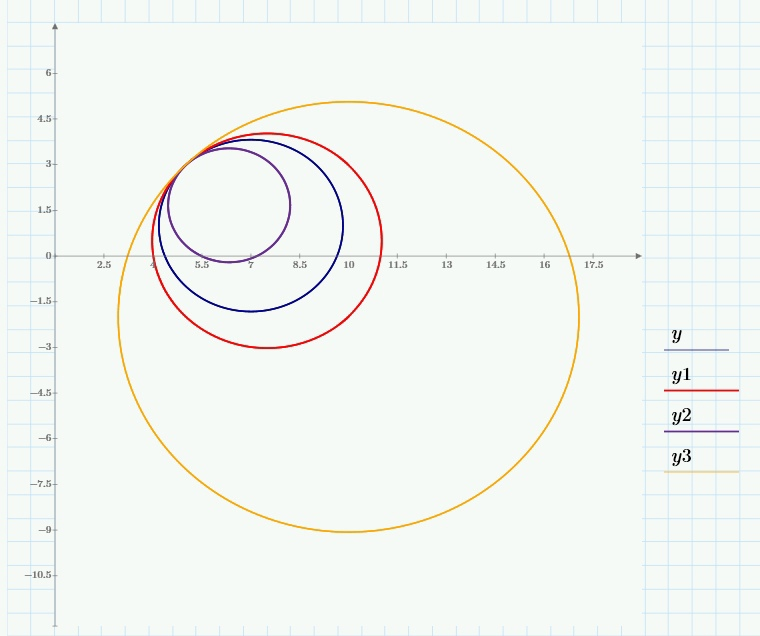
\includegraphics[width = \linewidth]{1.jpg}
			\caption{Траектории движения}
		\end{figure}
		\begin{figure}[H]
			\centering
			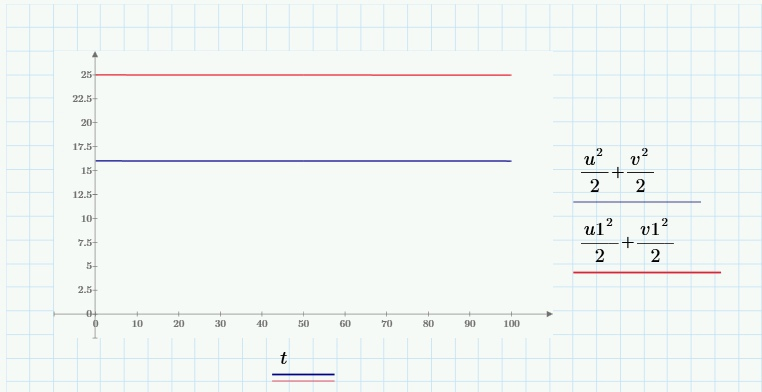
\includegraphics[width = \linewidth]{2.jpg}
			\caption{Графики зависимости $u^2+\upsilon^2$ от $t$}
		\end{figure}
		\begin{figure}[H]
			\centering
			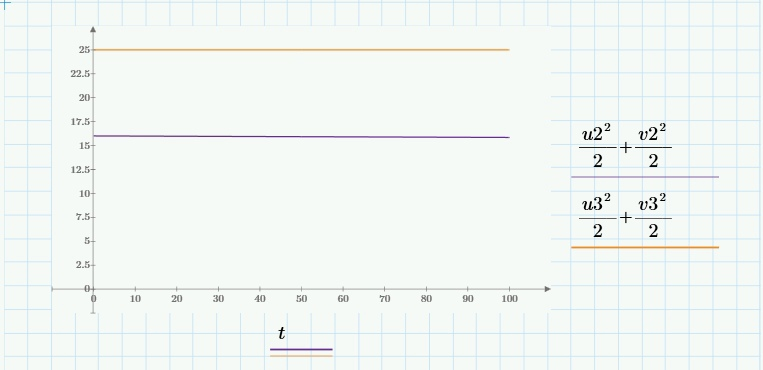
\includegraphics[width = \linewidth]{3.jpg}
			\caption{Графики зависимости $u^2+\upsilon^2$ от $t$}
		\end{figure}
		
	\section{Вывод}
		Была создана и реализована математическая модель движения тела во вращающейся системе координат.
		
\end{document}	